\documentclass[10pt]{article}
\usepackage{fullpage,enumitem,amsmath,amssymb,graphicx,listings,tikz,bbm,xcolor}
\setlength{\parindent}{0pt}

\begin{document}

\begin{center}
{\Large \textbf{Homework 8: From Language to Logic}}

\begin{tabular}{rl}
\\
Course: & CS 221 Spring 2019 \\
Name: & Bryan Yaggi
\end{tabular}
\end{center}

In this assignment, you will get some hands-on experience with logic. You'll see how logic can be used to represent the meaning of natural language sentences, and how it can be used to solve puzzles and prove theorems. Most of this assignment will be translating English into logical formulas, but in Problem 4, we will delve into the mechanics of logical inference.

\section*{\normalsize Problem 1: Propositional Logic}

\begin{enumerate}[label=(\alph*)]

	\item coding
	
	\item coding
	
	\item coding

\end{enumerate}

\section*{\normalsize Problem 2: First-Order Logic}

\begin{enumerate}[label=(\alph*)]

  \item coding
  
  \item coding
  
  \item coding
  
  \item coding

\end{enumerate}

\section*{\normalsize Problem 3: Liar Puzzle}

\begin{enumerate}[label=(\alph*)]

  \item coding

\end{enumerate}
\iffalse
\section*{\normalsize Problem 4: Particle Filtering}

\begin{enumerate}[label=(\alph*)]

  \item coding
  
  \item coding  

\end{enumerate}

\section*{\normalsize Problem 5: Which Car is It?}

So far, we have assumed that we have a distinct noisy distance reading for each car, but in reality, our microphone would just pick up an undistinguished set of these signals, and we wouldn't know which distance reading corresponds to which car. First, let's extend the notation from before: let $C_{ti} \in \mathbb{R}^2$ be the location of the $i$-th car at the time step $t$, for $i = 1, \dots, K$ and $t = 1, \dots, T$. Recall that all the cars move independently according to the transition dynamics as before.
\smallskip 

Let $D_{ti} \in \mathbb{R}$ be the noisy distance measurement of the $i$-th car, which is now not observed. Instead, we observe the set of distances $D_t = \{D_{t1}, \dots, D_{tK}\}$ (assume that all distances are all distinct). Alternatively, you can think of $E_t = (E_{t1}, \dots, E_{tK})$ as a list which is a uniformly random permutation of the noisy distances $(D_{t1}, \dots, D_{tK})$. For example, suppose $K = 2$ and $T = 2$. Before, we might have gotten distance readings of 1 and 2 for the first car and 3 and 4 for the second car. Now, our sensor readings would be permutations of $\{1, 3\}$ and $\{2 ,4\}$. Thus, even if we knew the second car was distance 3 away at time $t = 1$, we wouldn't know if it moved farther (4 away) or closer (2 away) at time $t = 2$.

\begin{enumerate}[label=(\alph*)]

  \item Suppose we have $K = 2$ cars and one time step $T = 1$. Write an expression for the conditional distribution $\mathbb{P}(C_{11}, C_{12} \mid E_1 = e_1)$ as a function of the PDF of a Gaussian $p_{\mathcal{N}}(\nu; \mu, \sigma^2)$ and the prior probability $p(c_{11})$ and $p(c_{12})$ over car locations. Your final answer should not contain variables $d_{11}$, $d_{12}$.
  
  Remember that $p_{\mathcal{N}}(\nu; \mu, \sigma^2)$ is the probability of a random variable, $\nu$, in a Gaussian distribution with mean $\mu$ and standard deviation $\sigma^2$. 
  
  \begin{center}
	  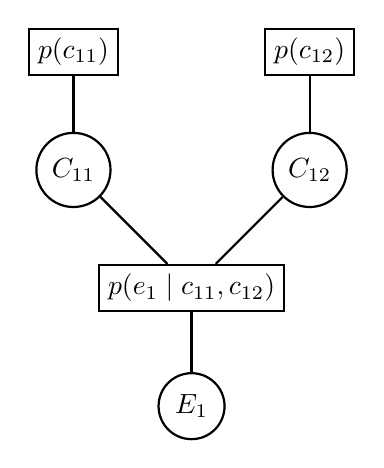
\begin{tikzpicture}
			\begin{scope}[every node/.style={circle,thick,draw}]
	    		\node (C11) at (0,0) {$C_{11}$};
	    		\node (C12) at (3,0) {$C_{12}$};
	    		\node (E1) at (1.5,-3) {$E_1$};
			\end{scope}
			\begin{scope}[every node/.style={rectangle,thick,draw}]
				\node (t0) at (0,1.5)	 {$p(c_{11})$};  		
	    		\node (t1) at (3,1.5) {$p(c_{12})$};
	    		\node (t2) at (1.5,-1.5) {$p(e_1 \mid c_{11}, c_{12})$};
			\end{scope}
			\begin{scope}[every edge/.style={draw=black,thick}]
				\path [-] (t0) edge node {} (C11);	    		
	    		\path [-] (t1) edge node {} (C12);
	    		\path [-] (C11) edge node {} (t2);
	    		\path [-] (C12) edge node {} (t2);
	    		\path [-] (t2) edge node {} (E1);
			\end{scope}
		\end{tikzpicture}
	\end{center}
	
	\begin{align*}
	\mathbb{P}(C_{11}, C_{12} \mid E_1 = e_1) &\propto p(c_{11}) p(c_{12}) (p(e_1 = \{ e_{11}, e_{12} \} \mid c_{11}, c_{12}) + p(e_1 = \{ e_{12}, e_{11} \} \mid c_{11}, c_{12}))\\
	p(e_1 = \{ e_{11}, e_{12} \} \mid c_{11}, c_{12}) &\propto p_{\mathcal{N}}(e_{11}; \lVert a_1 - c_{11} \rVert, \sigma^2) p_{\mathcal{N}}(e_{12}; \lVert a_1 - c_{12} \rVert, \sigma^2)\\
	p(e_1 = \{ e_{12}, e_{11} \} \mid c_{11}, c_{12}) &\propto p_{\mathcal{N}}(e_{12}; \lVert a_1 - c_{11} \rVert, \sigma^2) p_{\mathcal{N}}(e_{11}; \lVert a_1 - c_{12} \rVert, \sigma^2)\\
	\mathbb{P}(C_{11}, C_{12} \mid E_1 = e_1) &\propto p(c_{11}) p(c_{12}) (p_{\mathcal{N}}(e_{11}; \lVert a_1 - c_{11} \rVert, \sigma^2) p_{\mathcal{N}}(e_{12}; \lVert a_1 - c_{12} \rVert, \sigma^2)\\
	&+ p_{\mathcal{N}}(e_{12}; \lVert a_1 - c_{11} \rVert, \sigma^2) p_{\mathcal{N}}(e_{11}; \lVert a_1 - c_{12} \rVert, \sigma^2))
	\end{align*}
  
  \item Assuming the prior $p(c_{1i})$ is the same for all $i$, show that the number of assignments for all $K$ cars $(c_{11}, \dots, c_{1K})$ that obtain the maximum value of $\mathbb{P}(C_{11} = c_{11}, \dots, C_{1K} = c_{1K} \mid E_1 = e_1)$ is at least $K!$.
  
	Since the prior is the same for each car, each permutation of the initial assignment of observations to cars is also a solution. The total number of valid assignments is therefore $K!$.  
  
  \item For general $K$, what is the treewidth corresponding to the posterior distribution over all $K$ car locations at all $T$ time steps conditioned on all the sensor readings:
  $$\mathbb{P}(C_{11} = c_{11}, \dots, C_{1K} = c_{1K} , \dots, C_{T1} = c_{T1}, \dots, C_{TK} = c_{TK} \mid E_1 = e_1, \dots, E_T = e_T)$$

	The following factor graph shows 2 timesteps:
	
	\begin{center}
	  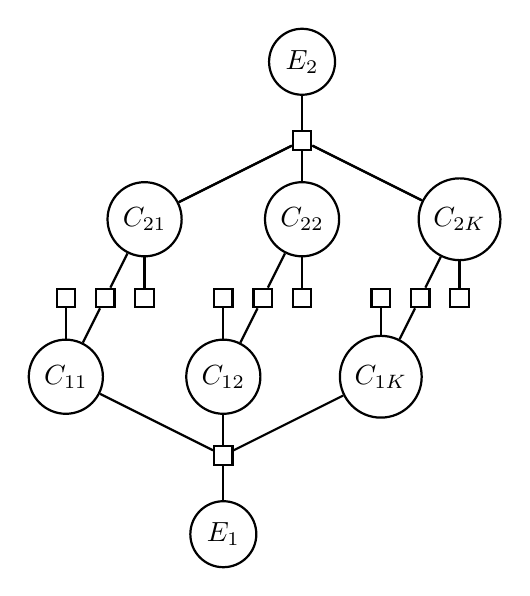
\begin{tikzpicture}
			\begin{scope}[every node/.style={circle,thick,draw}]
	    		\node (C11) at (0,0) {$C_{11}$};
	    		\node (C12) at (2,0) {$C_{12}$};
	    		\node (C1K) at (4,0) {$C_{1K}$};
	    		\node (E1) at (2,-2) {$E_1$};
	    		\node (C21) at (1,2) {$C_{21}$};
	    		\node (C22) at (3,2) {$C_{22}$};
	    		\node (C2K) at (5,2) {$C_{2K}$};
	    		\node (E2) at (3,4) {$E_2$};
			\end{scope}
			\begin{scope}[every node/.style={rectangle,thick,draw}]
				\node (t0) at (0,1)	 {};  		
	    		\node (t1) at (2,1) {};
	    		\node (t2) at (4,1) {};
	    		\node (t3) at (2,-1) {};
	    		\node (t4) at (1,1)	 {};  		
	    		\node (t5) at (3,1) {};
	    		\node (t6) at (5,1) {};
	    		\node (t7) at (3,3) {};
	    		\node (t8) at (.5,1) {};
	    		\node (t9) at (2.5,1) {};
	    		\node (t10) at (4.5,1) {};
			\end{scope}
			\begin{scope}[every edge/.style={draw=black,thick}]
				\path [-] (t0) edge node {} (C11);	    		
	    		\path [-] (t1) edge node {} (C12);
	    		\path [-] (t2) edge node {} (C1K);
	    		\path [-] (C11) edge node {} (t3);
	    		\path [-] (C12) edge node {} (t3);
	    		\path [-] (C1K) edge node {} (t3);
	    		\path [-] (t3) edge node {} (E1);
	    		\path [-] (t4) edge node {} (C21);	    		
	    		\path [-] (t5) edge node {} (C22);
	    		\path [-] (t6) edge node {} (C2K);
	    		\path [-] (C21) edge node {} (t7);
	    		\path [-] (C22) edge node {} (t7);
	    		\path [-] (C2K) edge node {} (t7);
	    		\path [-] (t5) edge node {} (C22);
	    		\path [-] (t6) edge node {} (C2K);
	    		\path [-] (C21) edge node {} (t7);
	    		\path [-] (C22) edge node {} (t7);
	    		\path [-] (C2K) edge node {} (t7);
	    		\path [-] (t7) edge node {} (E2);
	    		\path [-] (C11) edge node {} (t8);
	    		\path [-] (t8) edge node {} (C21);
	    		\path [-] (C12) edge node {} (t9);
	    		\path [-] (t9) edge node {} (C22);
	    		\path [-] (C1K) edge node {} (t10);
	    		\path [-] (t10) edge node {} (C2K);
			\end{scope}
		\end{tikzpicture}
	\end{center}
	
	The treewidth is $K$ as seen in the graph.
  
  \item \textbf{[Extra Credit]} Now suppose you change your sensors so that at each time step $t$, they return the list of exact positions of the $K$ cars, but shifted (with wrap around) by a random amount. For example, if the true car positions at time step 1 are $c_{11}=1$, $c_{12}=3$, $c_{13}=8$, $c_{14}=5$, then $e_1$ would be $[1,3,8,5]$, $[3,8,5,1]$, $[8,5,1,3]$, or $[5,1,3,8]$, each with probability $\frac{1}{4}$. Describe an efficient algorithm for computing $p(c_{ti} \mid e_1, \dots, e_T)$ for any time step $t$ and car $i$. Your algorithm should not be exponential in $K$ or $T$.
  
\end{enumerate}
\fi
\end{document}
